\documentclass[10pt,letterpaper]{article}

\usepackage[english]{babel}
\usepackage[utf8x]{inputenc}
\usepackage{amsmath}
\usepackage{graphicx}
\usepackage[colorinlistoftodos]{todonotes}

\usepackage{cite}
\usepackage{graphicx}
\usepackage{float}

\title{Monte Carlo Simulation of Ising Model Lattice}
\author{Stephen Mee}

\begin{document}
\maketitle

\begin{abstract}

Using the Wolff algorithm for a range of temperature values, the critical temperature and other macroscopic and microscopic values are found for a two-dimensional lattice of electron spin states.

\end{abstract}

\section{Introduction}

A two-dimensional lattice of electron spin states is initialized. For each temperature value, a random site is chosen and added to the cluster specified in the Wolff algorithm. Using periodic boundary conditions, the 4 nearest neighbors of the chosen site are added to a "queue" if they pass an exponential check. The sites that are in the queue are subsequently added to the cluster and the algorithm to add their nearest neighbors is run again. Sites that have been added to the cluster immediately have the sign of their spin flipped.

After a predetermined number of clusters are built on the lattice, a range of values are calculated and plotted vs. temperature. These values include: magnetization, critical temperature, magnetic susceptibility, internal energy, heat capacity, and critical exponents of the magnetization near the critical temperature.

\section{Wolff Algorithm}

The Wolff algorithm relies on the idea of flipping entire "clusters" of spin states at once, as opposed to the Metropolis algorithm which only flips individual states. The condition to add sites to the cluster is as follows:

\begin{equation}
R < 1 - \exp\frac{-2J}{k_{b}T}
\end{equation}

Where $R$ is a number picked from a random distribution ranging from 0 to 1, $J$ is the coupling constant, $k_{B}$ is the Boltzmann constant, and $T$ is the temperature. In the code, both $J$ and $k_{B}$ have arbitrarily been set to one.

The size of the cluster is a function of temperature; for low temperatures we expect the cluster to encompass the entire lattice while for high temperatures we expect the clusters to be much smaller. Because of this temperature dependence, the number of clusters being built on a single lattice also needs be a function of temperature to ensure accurate results. Each cluster will sample less at high temperatures, so more clusters will be needed to cover the entire lattice. A temperature-dependent cluster number has been built into the code to compensate for this.



\section{Code Results}

All results were found with a lattice of N = 22500 that was initialized with all spin-up sites. The temperature ranged from T = 0.01K - 4.0K in iterations of 0.01K. From 0.01K - 2.0K there are 10 clusters built per lattice, 2.01K - 2.5K there are $2*\sqrt[]{N}$, and from 2.51K - 4.0K there are $2N$. The cluster process is repeated 20 times for any given temperature to get an average magnetization and calculate the standard deviation.

\subsection{Magnetization}

The magnetization is found by:

\begin{equation}
M = \frac{1}{N} \sum_{i}\sum_{j}{S_{i,j}}
\end{equation}

Where $S_{i,j}$ is the spin state of the $[i,j]$ index of the electron lattice. The magnetization is expected to stay near one for low temperatures then plummet to zero near the "critical temperature", following a roughly S-shaped curve.

\begin{figure}[H]
\centering
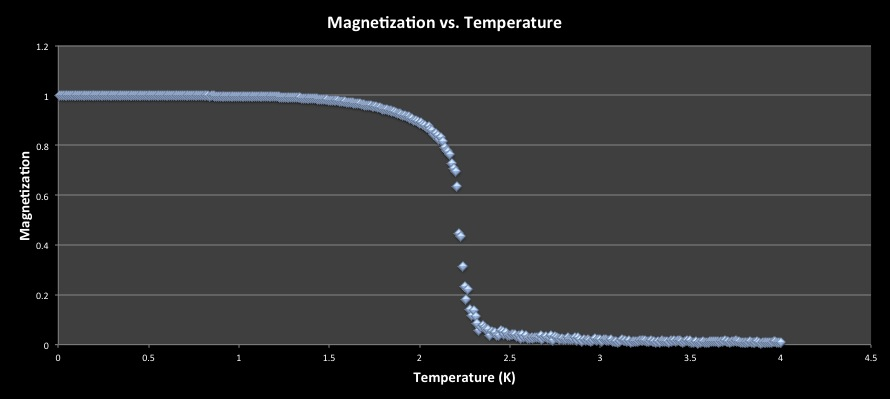
\includegraphics[width=120mm]{Magnetization.jpg}
\caption{Magnetization versus temperature for N = 22500}
\end{figure}

\pagebreak

\subsection{Magnetic Susceptibility}

The susceptibility is defined as: 

\begin{equation}
\chi = \frac{\partial{M}}{\partial{T}}
\end{equation}

Assuming many temperature iterations, this can approximated as:

\begin{equation}
\chi = \frac{\Delta{M}}{\Delta{T}} = \frac{M_{n+1} - M_{n}}{T_{n+1} - T_{n}}
\end{equation}

Based off the plot for magnetization one would expect the susceptibility to look like a sharp Gaussian in the negative direction, with the peak located at the point where the magnetization was most rapidly changing. 

\begin{figure}[H]
\centering
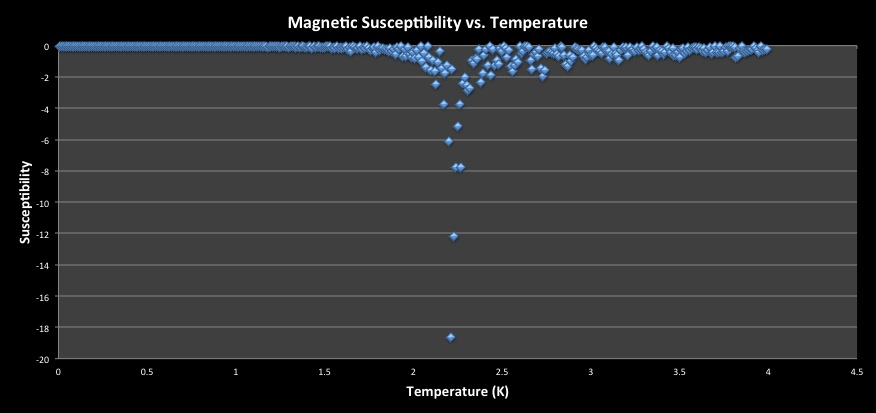
\includegraphics[width=120mm]{Susceptibility.jpg}
\caption{Magnetic Susceptibility vs Temperature for N = 22500}
\end{figure}

\subsection{Internal Energy}

The internal energy is defined as:

\begin{equation}
E = - J \sum_{i,NN}S_{i}S_{NN}
\end{equation}

Where $J$ is the coupling constant, $S_{i}$ is a single spin, and $S_{NN}$ is representative of the spins of the nearest neighbors of $S_{i}$. 

When summing over all indexes the algorithm must be careful to not double-count the same interaction. This was bypassed by only considering a single horizontal and vertical neighbor for any given particle. Assuming periodic boundary conditions, summing over all $S_{i}$ using this method manages to include all nearest neighbor interactions. 

\begin{figure}[H]
\centering
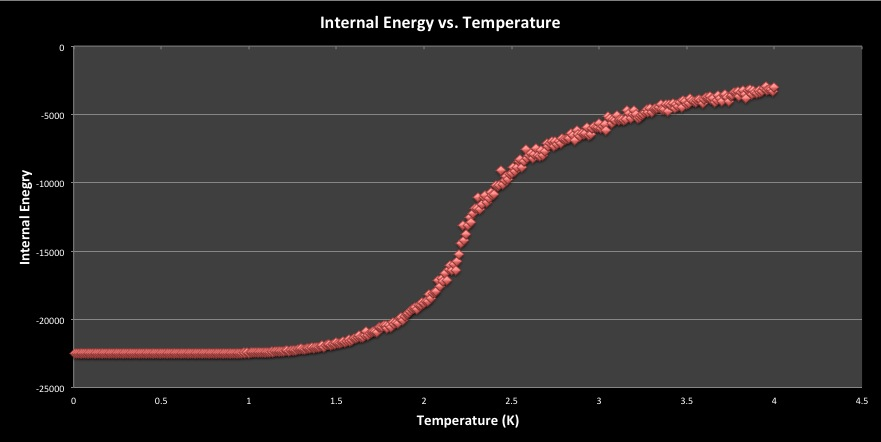
\includegraphics[width=120mm]{InternalEnergy.jpg}
\caption{Internal Energy vs Temperature for N = 22500}
\end{figure}

\subsection{Heat Capacity}

The heat capacity is defined as:

\begin{equation}
C = \frac{\partial{E}}{\partial{T}}
\end{equation}

Similarly to the susceptibility, this can be rewritten as:

\begin{equation}
C = \frac{\Delta{E}}{\Delta{T}} = \frac{E_{n+1} - E_{n}}{T_{n+1} - T{n}}
\end{equation}

Once again, the heat capacity would be expected to be a Gaussian in the positive direction with the peak at the moment of the most rapid change.

\begin{figure}[H]
\centering
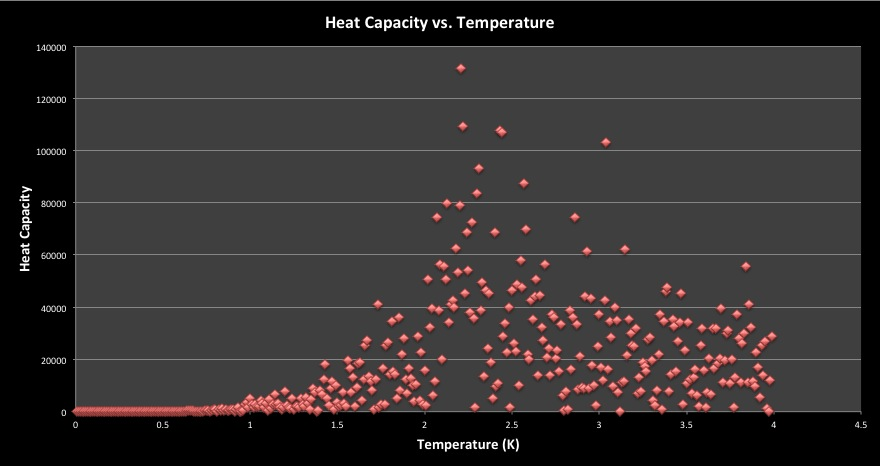
\includegraphics[width=120mm]{HeatCapacity.jpg}
\caption{Heat Capacity versus Temperature for N = 22500}
\end{figure}

\subsection{Critical Temperature}

The critical temperature can be defined as both the point at which the magnetization and the internal energy are most rapidly changing. Equivalently, we are looking for the temperature where the concavity of the magnetization and internal energy switches sign. This is written mathematically as:

\begin{equation}
0 = \frac{\partial^{2}M}{\partial{T}^{2}}
\end{equation}

\begin{equation}
0 = \frac{\partial^{2}E}{\partial{T}^{2}}
\end{equation}

By solving for T in both cases, we can conclude:

\begin{equation}
T_{c} \approx 2.21K
\end{equation}

This is supported by the simulation. Without averaging the magnetization over many runs, 2.2K is approximately when the calculated values began to fluctuate wildly. The statistical noise after the simulation passes the critical temperature is still readily apparent in Figure 4. 

\subsection{Critical Exponents}

It was decided that the calculation of the critical exponent $\gamma$ for the magnetization would yield the cleanest results. Around the critical temperature, the magnetization obeys the following power law:

\begin{equation}
M = |T - T_{c}|^{\gamma}
\end{equation}

Which can be rewritten as:

\begin{equation}
\gamma = \frac{\ln(M)}{\ln(|T - T_{c}|)} = \ln(M - |T - T_{c}|)
\end{equation}

The calculation of gamma requires a lot of precise data in the region surrounding the critical temperature. Because of this, it was decided the original run would not provide good enough statistics. A second simulation run was preformed with N = 22500, $T_{init}$ = 2.18K, $T_{end}$ = 2.24K, and $T_{iter}$ = 0.002K to provide better data. The gamma values calculated for each temperature iteration are as follows:

\begin{figure}[H]
\centering
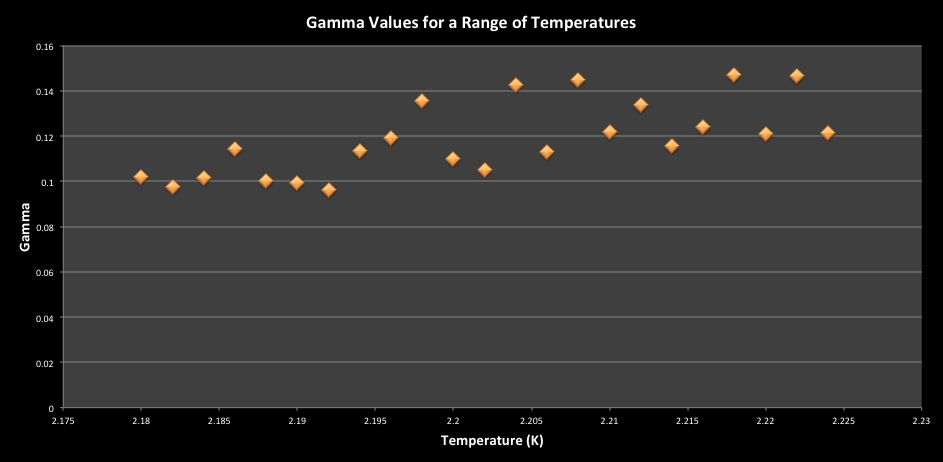
\includegraphics[width=120mm]{GammaValues.jpg}
\caption{A range of calculated gamma values around the critical temperature}
\end{figure}

After the simulation passes the critical temperature the gamma values begin to fluctuate, so only temperature values up to 2.224K are plotted above. By taking the average of all the above values above we can estimate:

\begin{equation}
\gamma = 0.119 \approx 0.125
\end{equation}

Which is the accepted value of the critical index.

\section{Conclusion}

The Wolff algorithm provides more concise and accurate data for low temperatures at the expense of accuracy at high temperatures. For the same effective input the Wolff algorithm also runs faster than the Metropolis algorithm, but suffers from being a much more specific model that cannot apply to many other cases.

At high temperatures the clusters become very small (single sites), and the Wolff Algorithm devolves into the Metropolis algorithm. Because of this more clusters must be run at high temperatures for accurate.

Overall this simulation produces results consistent with the Metropolis algorithm simulation and the theory behind the Ising model. The Ising model predicts a critical temperature $T_{C}$ around 2.27K, very close to the calculated 2.21K. Below are plots of magnetization and heat capacity calculated by Nikos Drakos from the University of Leeds and Ross Moore from Macquarie University. Both plots can be seen to match the results presented in this report.

\begin{figure}[H]
\centering
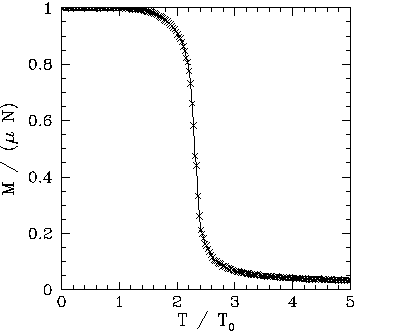
\includegraphics[width=50mm]{UTexasMagnetization.jpg}
\caption{Drakos, Nikos, and Ross Moore. Figure 115. Digital image. University of Texas, 29 Mar. 2006. Web. 31 Mar. 2015. <http://farside.ph.utexas.edu/teaching/329/lectures/node110.html>}
\end{figure}

\begin{figure}[H]
\centering
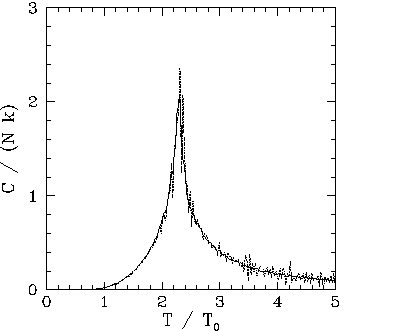
\includegraphics[width=50mm]{UTexasHeatCapacity.png}
\caption{Drakos, Nikos, and Ross Moore. Figure 116. Digital image. University of Texas, 29 Mar. 2006. Web. 31 Mar. 2015. <http://farside.ph.utexas.edu/teaching/329/lectures/node110.html>.}
\end{figure}











\end{document}